% =============================================================================
% DiD-BCF revision: complete interim simulation report
% Current full structured grid plus the partial unit-random-intercept route audit.
% =============================================================================
\documentclass[11pt]{article}

\usepackage[a4paper,margin=2.5cm]{geometry}
\usepackage{amsmath,amssymb,mathtools}
\usepackage{booktabs}
\usepackage{array}
\usepackage{longtable}
\usepackage{graphicx}
\usepackage{microtype}
\usepackage[hidelinks]{hyperref}

\newcommand{\att}{\mathrm{ATT}}
\newcommand{\gatt}{\mathrm{GATT}}
\newcommand{\es}{\mathrm{ES}}
\newcommand{\catt}{\mathrm{CATT}}
\newcommand{\ind}{\mathbb{1}}

\graphicspath{{figures/}}

\title{\textbf{Forests for Differences}: complete interim simulation results for DiD-BCF}
\author{Simulation report}
\date{1 August 2026}

\begin{document}
\maketitle

\begin{abstract}
This report reanalyzes the complete set of currently available simulation
summaries after the identification and design corrections. The main full-grid
analysis covers the structured DiD-BCF specification in all available B1, B2,
and D designs at linearity degrees $d=1,2,3$. The B1 designs include the
baseline, strong-confounder, serial-correlation, selection-on-observables, and
sharp-null cases. The B2 designs contain the ordinary and serial-correlation
sample-size sweeps. The D designs contain staggered adoption and its stronger
contamination variant. Each available full-grid cell has 100 replications,
except for the 200-replication TWFE null benchmark.

The report also analyzes the separate post-correction route file, which is the
only current file containing both structured DiD-BCF and structured DiD-BCF with
a unit-level random intercept. That route audit covers the B2 ordinary sweep
at $d=1$, with 15 replications per panel size and $N\in\{200,400,800,1600\}$.
Both specifications are called DiD-BCF throughout, with the unit-intercept
column identifying the implementation.

The complete structured grid shows small scalar bias in the B1 and B2 designs,
stable performance across the corrected $d=2$ and $d=3$ axes for the plain
structured fit, and strong performance on the staggered cohort-time targets.
The posterior correction improves uncertainty calibration in the serial and
staggered designs at $d=1$, but that advantage does not survive the nonlinear
nuisance axis: at $d=2$ and $d=3$ its event-study RMSE in the staggered designs
exceeds pooled TWFE at every event time. Under the sharp null both DiD-BCF
specifications are correctly sized, the plain fit conservatively so. The
staggered results reject the use of pooled TWFE as the main heterogeneous
effect benchmark. The two covariate-adaptive benchmarks, DoubleML DR-DiD and
grf-DiD (Wang), are reported over the full degree axis in every design in which
they were run, and both prove nearly invariant to the nonlinear nuisance axis,
which makes them the fixed reference against which the DiD-BCF degree
sensitivity is read. The partial unit-intercept route has a small surface-RMSE
advantage over the no-unit-intercept implementation in the B2 $d=1$ audit,
but it has not yet been run over the remaining DGPs or degrees.
\end{abstract}

\tableofcontents

% =============================================================================
\section{Scope, result files, and coverage}
% =============================================================================

The report distinguishes the complete current structured grid from the newer
route-comparison file. The complete grid is read from
\begin{center}
\url{DiD_BCF/summaries_B1_*.csv},\quad
\url{DiD_BCF/summaries_B2_*.csv},\quad
\url{DiD_BCF/summaries_D_*.csv}.
\end{center}
These are tidy per-replication summaries with both \texttt{plain} and
\texttt{corrected} methods and the single specification field
\texttt{structured}. The summary files cover every listed B1 and D design at
$d=1,2,3$, and both B2 sweeps at every panel size
$N\in\{50,100,200,400,800\}$ and degree $d\in\{1,2,3\}$. The absence of a
file is treated as missing coverage, not as a zero or as a completed sweep.

The route-comparison file is
\begin{center}
\url{Results/identification/routes_raw_B2_sweep_lin_1_full.csv}\par
\url{Results/identification/routes_summary_B2_sweep_lin_1_full.csv}
\end{center}
It contains several identification routes, but this report retains only
\begin{center}
\texttt{structured}\qquad \texttt{structured\_rfx\_unit}
\end{center}
The first is the two-way-restricted DiD-BCF fit without a unit random
intercept. The second is the same fit with an additive unit-level random
intercept. The route file has
15 replications per method, panel size, and method summary. It is not pooled
with the 100-replication full-grid summaries.

The benchmark summaries were rebuilt from the current files in
\begin{center}
\url{R_code/}\qquad \url{Results/_staging/DoubleML_Colab/}\qquad
\url{Results/_staging/CFFE_Wang_Colab/}
\end{center}
and the current TWFE summaries in \url{Results/summaries_twfe_*.csv}. The
folder named \texttt{CFFE\_Wang\_Colab} contains the grf-DiD implementation
associated with Wang, so it is labelled grf-DiD (Wang) rather than CFFE in the
tables. The benchmark availability by scenario and panel size is shown in
Table~\ref{tab:grid}; the table was regenerated from the actual files before
this report was written.

\begingroup
\setlength{\tabcolsep}{0.5pt}
\input{tables/tab_grid.tex}
\endgroup

Two benchmark estimators are reported over the full degree axis in every design
in which they were run. DoubleML DR-DiD covers all five B1 designs, both D
designs, and all five panel sizes of both B2 sweeps, at $d=1,2,3$. grf-DiD
(Wang) covers all five B1 designs, both D designs, and all five panel sizes of
both B2 sweeps, at $d=1,2,3$. Because
both estimators report cohort-time effects rather than a pooled ATT or an
event-study coefficient, they appear in the $\gatt$ tables rather than in the
ATT table, and in the staggered designs they are read cell by cell.

The full grid does not yet contain a completed B1 selection-on-both result,
although that design is defined in the DGP code and is described below. It is
therefore not silently included as if it had been run. Likewise, the unit
random-intercept route is not presented for B1, B2 serial correlation, or D,
because no corresponding route summaries are currently present.

% =============================================================================
\section{Mathematical simulation design}
% =============================================================================

\subsection{Persistent latent covariates and the degree axis}

Each replication draws persistent unit-level covariates once and carries them
through the $T=8$ periods. For unit $i=1,\ldots,N$,
\begin{equation}
 X_{1i}\sim\operatorname{Bernoulli}(0.5),\qquad
 (X_{2i},X_{3i},X_{4i})\sim\mathcal{N}(0,1)^3,\qquad
 X_{5i}\sim\operatorname{Uniform}(-1,1),
 \label{eq:covariates}
\end{equation}
with independent draws across units. At $d=1$ the estimator receives the
latent covariates. At $d=2$ and $d=3$ the DGP remains a function of the same
latent variables, but the estimator receives
\begin{align}
 X_{1i}^{o}&=X_{1i}, & X_{2i}^{o}&=X_{2i},\\
 X_{3i}^{o}&=\operatorname{std}\!\left[
       \left(\frac{X_{3i}X_{4i}}{5}+0.6\right)^3\right], &
 X_{4i}^{o}&=\operatorname{std}\!\left[\exp(X_{4i}/2)\right],\\
 X_{5i}^{o}&=\operatorname{std}\!\left[(X_{3i}+X_{5i}+2)^2\right].
 \label{eq:ks-transforms}
\end{align}
Here standardisation is within replication. Thus $d=2$ changes the
parameterisation of the nuisance functions without changing the true outcome
or estimands. At $d=3$, the treatment-effect surface is also changed from an
additive linear function to a centered quadratic and interaction while its
mean and variance are held fixed.

\subsection{Canonical B1 and B2 designs}

Let $A_i\sim\mathcal{N}(0,1)$ and let the unobserved time-invariant unit
effect be
\begin{equation}
 \alpha_i=\sigma_\alpha A_i.
 \label{eq:alpha}
\end{equation}
The assignment utility is
\begin{equation}
 U_i=
 \begin{cases}
  0.8X_{1i}+0.6X_{4i}, & \text{selection on observables},\\
  c_\alpha A_i, & \text{selection on the unobservable},\\
  0.8X_{1i}+0.6X_{4i}+c_\alpha A_i, & \text{selection on both}.
 \end{cases}
 \label{eq:utility}
\end{equation}
The utility is centered at the target treated share $p_T=0.5$, and treatment
is drawn from
\begin{equation}
 T_i\mid X_i,A_i\sim
 \operatorname{Bernoulli}\!\left[
 \operatorname{logit}^{-1}\!\left(
 1.5\left[U_i-Q_{1-p_T}(U)\right]+\nu_i
 \right)\right],
 \qquad \nu_i\sim\mathcal{N}(0,0.5^2).
 \label{eq:assignment}
\end{equation}
For the canonical designs, treated units adopt at $G_i=4$ and never-treated
units have $G_i=\infty$. With $t=0,\ldots,7$,
\begin{equation}
 D_{it}=\ind\{G_i\le t\},
 \qquad k_{it}=t-G_i.
 \label{eq:canonical-treatment}
\end{equation}

The untreated potential outcome is
\begin{equation}
 Y_{it}(0)=\beta_0+\alpha_i+\gamma_t+f(X_i)+s(X_i)t+\varepsilon_{it},
 \label{eq:untreated}
\end{equation}
where
\begin{align}
 \beta_0&=-0.5, & \gamma_t&=0.2t,\\
 f(X_i)&=-0.75X_{1i}+0.5X_{2i}-0.5X_{3i}-1.3X_{4i}+1.8X_{5i},\\
 s(X_i)&=0.3\left(0.7X_{4i}+\sqrt{0.51}X_{3i}\right).
 \label{eq:canonical-components}
\end{align}
The observed outcome is
\begin{equation}
 Y_{it}=Y_{it}(0)+D_{it}\tau_i.
 \label{eq:canonical-outcome}
\end{equation}
For $d\in\{1,2\}$, the heterogeneous effect is
\begin{equation}
 \tau_i=3+1.5X_{1i}+0.75X_{2i}.
 \label{eq:tau-linear}
\end{equation}
For $d=3$, it is
\begin{equation}
 \tau_i=3+1.5X_{1i}+0.75\left[
 \frac{1}{\sqrt{2}}\left\{
 \frac{X_{2i}^2-1}{\sqrt{2}}+(2X_{1i}-1)X_{2i}
 \right\}\right].
 \label{eq:tau-nonlinear}
\end{equation}
The null design sets $\tau_i=0$ for every unit. Serial-correlation designs
replace iid errors by the stationary AR(1) process
\begin{equation}
 \varepsilon_{it}=\rho\varepsilon_{i,t-1}
 +\sigma_\varepsilon\sqrt{1-\rho^2}\,Z_{it},
 \qquad Z_{it}\sim\mathcal{N}(0,1).
 \label{eq:ar1}
\end{equation}

The canonical scenario settings used by the current summaries are
\begin{center}
\begin{tabular}{lrrrrl}
\toprule
Scenario & $\sigma_\alpha$ & $c_\alpha$ & Selection & $\rho$ & Effect \\
\midrule
\texttt{B1\_baseline} & 1 & 1 & unobservable & 0 & heterogeneous \\
\texttt{B1\_strong\_confounder} & 2 & 1.5 & unobservable & 0 & heterogeneous \\
\texttt{B1\_serial\_corr} & 1 & 1 & unobservable & 0.6 & heterogeneous \\
\texttt{B1\_selection\_obs} & 1 & 0 & observable & 0 & heterogeneous \\
\texttt{B1\_null} & 1 & 1 & unobservable & 0 & zero \\
\texttt{B2\_sweep} & 1 & 1 & unobservable & 0 & heterogeneous \\
\texttt{B2\_sweep\_serial} & 1 & 1 & unobservable & 0.6 & heterogeneous \\
\bottomrule
\end{tabular}
\end{center}
The B1 designs use $N=200$. Both B2 sweeps contain structured DiD-BCF cells at
$N\in\{50,100,200,400,800\}$. The DoubleML and Wang benchmark files now cover
the same five panel sizes, and additionally retain a stale $N=1600$ column from
before that size was dropped; the remaining benchmark availability is shown in
Table~\ref{tab:grid}.

\subsection{Staggered D designs}

The D designs assign units to adoption cohorts $G_i\in\{4,5,6,\infty\}$,
with shares $(0.25,0.25,0.25,0.25)$. Cohort assignment uses a multinomial
Gumbel draw. Let $s_0$ denote the never-treated share, let $s_j$ denote the
share of treated cohort $j$, and let $q_i$ be the selected observable,
unobservable, or combined assignment driver. The utilities are
\begin{align}
 V_{i0}&=\log(s_0)+\xi_{i0},\\
 V_{ij}&=\log(s_j)+\left[0.8+0.5\left(1-\frac{j-1}{K-1}\right)\right]q_i+\xi_{ij},
 \qquad \xi_{ij}\sim\operatorname{Gumbel}(0,1),
 \label{eq:cohort-assignment}
\end{align}
and the selected cohort maximizes $V_{ij}$. For cohort $g_j$ and event time
$k=t-g_j\ge0$, the effect is
\begin{equation}
 \tau_{it}(g_j,k)=M_j(1+rk)\tau_i,
 \label{eq:staggered-effect}
\end{equation}
so that
\begin{equation}
 Y_{it}=Y_{it}(0)+D_{it}\tau_{it}(G_i,k_{it}).
 \label{eq:staggered-outcome}
\end{equation}
The headline staggered design uses
$(M_1,M_2,M_3)=(1,1.5,2)$ and $r=0.4$. The contamination design uses
$(M_1,M_2,M_3)=(1,2,3)$ and $r=0.8$. These two designs deliberately create
cohort and event-time heterogeneity, the setting in which already-treated-as-
control comparisons contaminate pooled TWFE.

% =============================================================================
\section{Estimands and estimators}
% =============================================================================

\subsection{True estimands}

The individual treatment effect on a treated post-treatment observation is
\begin{equation}
 \catt_{it}=D_{it}\tau_{it},
 \label{eq:catt}
\end{equation}
where $\tau_{it}=\tau_i$ in the canonical designs and
Equation~\eqref{eq:staggered-effect} applies in the D designs. For a cohort $g$
and calendar time $t$,
\begin{equation}
 \gatt(g,t)=\frac{1}{n_{g,t}}
 \sum_{i:G_i=g}\catt_{it}.
 \label{eq:gatt}
\end{equation}
The event-study estimand is
\begin{equation}
 \es(k)=\frac{1}{n_k}
 \sum_{i,t:G_i<\infty,\,t-G_i=k}\catt_{it},
 \label{eq:event-study}
\end{equation}
and the overall treated-post ATT is
\begin{equation}
 \att=\frac{1}{n_1}\sum_{i,t:D_{it}=1}\catt_{it}.
 \label{eq:att}
\end{equation}
In the single-cohort designs, $\gatt(4,4)$, $\es(0)$, and the overall ATT
target the same post-treatment average, although the estimators report them
through different interfaces. In the D designs, cohort and event time matter,
so the GATT and event-study results must be read cell by cell.

\subsection{DiD-BCF specifications}

Both structured implementations are reported as DiD-BCF. The common model is
\begin{equation}
 Y_{it}=a(G_i,X_i)+b(t,X_i)
 +\left\{\tau_0+\tau(X_i,k_{it},G_i)\right\}D_{it}+u_i+\varepsilon_{it}.
 \label{eq:structured-model}
\end{equation}
For the structured implementation without a unit intercept, $u_i=0$. For
structured DiD-BCF with a unit random intercept, $u_i$ is an additive,
time-invariant random effect indexed by unit. The level forest $a$ receives
the cohort label and covariates but no time column. The trend forest $b$
receives calendar time and covariates but no cohort label. The treatment forest
receives the effect modifiers, event time, and cohort when cohort-specific
effects are needed. This is the structural two-way restriction
\begin{equation}
 \mu(G_i,t,X_i)=a(G_i,X_i)+b(t,X_i),
 \label{eq:two-way}
\end{equation}
which prevents the prognostic component from representing a group-by-time
treatment interaction. The unit intercept cancels in a time difference and
therefore does not reopen that interaction; it additionally absorbs persistent
unit-level outcome heterogeneity.

The plain DiD-BCF estimand is the posterior treatment forest evaluated on
treated post-treatment observations. The corrected estimand uses the fitted
untreated change. For cohort $g$ compared with never-treated units, define
\begin{equation}
 \delta_i=\ind\{G_i=g\},\qquad
 \Delta Y_i=Y_{it}-Y_{i,g-1},\qquad
 m_i^s=\mu_i^s(t)-\mu_i^s(g-1).
 \label{eq:correction-inputs}
\end{equation}
Let $\widehat\pi_i$ estimate $P(\delta_i=1\mid X_i)$ and let
\begin{equation}
 \widehat\gamma_i=\frac{\delta_i-\widehat\pi_i}
 {(1-\widehat\pi_i)\overline\pi},
 \qquad
 A_i=\delta_i-(1-\delta_i)\frac{\widehat\pi_i}{1-\widehat\pi_i}.
 \label{eq:correction-weights}
\end{equation}
With Bayesian-bootstrap weights $W_i^s$, the corrected draw is
\begin{align}
 \widehat\theta_{g,t}^s
 &=\frac{\sum_iW_i^sA_i(\Delta Y_i-m_i^s)}
 {\sum_iW_i^s\delta_i},\\
 \widehat b_{g,t}^s
 &=\frac{1}{n_g}\sum_i\widehat\gamma_i(\overline m_i-m_i^s),\\
 \widetilde\theta_{g,t}^s
 &=\widehat\theta_{g,t}^s-\widehat b_{g,t}^s,
 \qquad \overline m_i=\frac{1}{S}\sum_{s=1}^S m_i^s.
 \label{eq:posterior-correction}
\end{align}
The corrected point estimate and interval are the posterior mean and empirical
quantiles of the corrected draws. Aggregated ATT and event-study draws use
treated-count weights over the relevant cohort-time cells.

\subsection{Benchmark estimators}

The comparison includes TWFE, Callaway--Sant'Anna's doubly robust group-time
estimator, Gardner's two-stage event-study estimator, Synthetic DiD, the
DoubleML doubly robust DiD estimator, and grf-DiD (Wang). The GATT-only
estimators are broadcast to treated observations when the individual CATT
surface is evaluated. This is a deliberately transparent benchmark: it gives
cell-level estimators their natural scalar prediction while preserving the
distinction between scalar identification and individual heterogeneity.

% =============================================================================
\section{Evaluation formulas}
% =============================================================================

Let $\widehat\theta_r$ be the estimate in replication $r$, let $\theta_r$ be
the replication-specific realised target, and let
$e_r=\widehat\theta_r-\theta_r$. The main scalar metrics are
\begin{align}
 \operatorname{Bias}&=\frac{1}{R}\sum_{r=1}^R e_r,\\
 \operatorname{RMSE}&=\left(\frac{1}{R}\sum_{r=1}^R e_r^2\right)^{1/2},\\
 \operatorname{MAE}&=\frac{1}{R}\sum_{r=1}^R|e_r|,\\
 \operatorname{MAPE}&=\frac{1}{|\mathcal{R}_+|}
 \sum_{r\in\mathcal{R}_+}\left|\frac{e_r}{\theta_r}\right|,
 \qquad \mathcal{R}_+=\{r:|\theta_r|>10^{-8}\}.
 \label{eq:scalar-metrics}
\end{align}
Because the target itself varies across replications, the tables also report
the Monte-Carlo standard deviation of the estimation error,
\begin{align}
 \operatorname{SD}(e)&=\left[\frac{1}{R-1}\sum_{r=1}^R
 (e_r-\overline e)^2\right]^{1/2},\\
 \operatorname{SD}_{\mathrm{table}}(e)&=
 \left[\operatorname{RMSE}^2-\operatorname{Bias}^2\right]^{1/2}.
 \label{eq:error-sd}
\end{align}
For an interval $[L_r,U_r]$,
\begin{align}
 \operatorname{Coverage}_{1-\alpha}
 &=\frac{1}{R}\sum_{r=1}^R
 \ind\{L_r\le\theta_r\le U_r\},\\
 \operatorname{Length}_{1-\alpha}
 &=\frac{1}{R}\sum_{r=1}^R(U_r-L_r),\\
 \operatorname{SDRatio}&=\frac{R^{-1}\sum_{r=1}^R s_r}
 {\operatorname{SD}(\widehat\theta)}.
 \label{eq:coverage}
\end{align}
Here $s_r$ is the reported posterior standard deviation or standard error. The
Monte-Carlo standard errors of the bias and coverage are
\begin{equation}
 \operatorname{MCSE}(\operatorname{Bias})
 =\frac{\operatorname{SD}(\widehat\theta)}{\sqrt R},
 \qquad
 \operatorname{MCSE}(\operatorname{Coverage})
 =\left[\frac{\widehat p(1-\widehat p)}{R}\right]^{1/2}.
 \label{eq:mcse}
\end{equation}

For the individual effect surface, let $\widehat\catt_{ir}$ be the prediction
for treated observation $i$ in replication $r$ and let
$n_r^{\mathrm{tr}}$ be the number of treated post-treatment observations.
The within-replication surface metrics are
\begin{align}
 \operatorname{RMSE}_{\mathrm{surf},r}
 &=\left[\frac{1}{n_r^{\mathrm{tr}}}
 \sum_{i:D_{ir}=1}(\widehat\catt_{ir}-\catt_{ir})^2\right]^{1/2},\\
 \operatorname{MAE}_{\mathrm{surf},r}
 &=\frac{1}{n_r^{\mathrm{tr}}}
 \sum_{i:D_{ir}=1}|\widehat\catt_{ir}-\catt_{ir}|,\\
 \operatorname{MAPE}_{\mathrm{surf},r}
 &=\frac{1}{|\mathcal{I}_r|}
 \sum_{i\in\mathcal{I}_r}
 \left|\frac{\widehat\catt_{ir}-\catt_{ir}}{\catt_{ir}}\right|,
 \quad \mathcal{I}_r=\{i:D_{ir}=1,|\catt_{ir}|>10^{-8}\}.
 \label{eq:surface-metrics}
\end{align}
The reported surface values average these within-replication quantities over
replications. Finally, the finite-sample rate diagnostic is
\begin{equation}
 Z_r=\sqrt{N}(\widehat\theta_r-\theta_r),
 \label{eq:sqrt-n}
\end{equation}
whose mean should approach zero and whose standard deviation should stabilize
for a valid $\sqrt N$ approximation.

% =============================================================================
\section{Coverage and complete-grid results}
% =============================================================================

\subsection{B1 scalar estimands}

The decomposed ATT results are reported in Table~\ref{tab:b1att}, and the
directly comparable $\gatt(4,4)$ results are in Table~\ref{tab:b1gatt}.
DoubleML DR-DiD and grf-DiD do not appear in the ATT table because neither
reports a pooled ATT; both report cohort-time effects, so their canonical-design
results are in Table~\ref{tab:b1gatt}, at all three degrees. At
$d=1$, the structured DiD-BCF point estimates are close to the true target in
the baseline, strong-confounder, serial-correlation, and selection-on-
observables designs. The plain specification is especially stable in the
baseline and strong-confounder cases. The corrected specification generally
has a larger posterior spread, which is useful under serial correlation but
can become costly under transformed covariates.

The degree axis is now informative. The $d=2$ and $d=3$ plain structured
estimates remain close to zero in the canonical scalar comparisons, although
their uncertainty calibration deteriorates in the serial and selection-on-
observables settings. The corrected summaries show much larger RMSE and
reported-spread distortions at $d=2$ and $d=3$, especially under
selection-on-observables. This is evidence about the current posterior
correction implementation and sampler budget, not evidence that the DGP has
become unidentified: the DGP truth is unchanged at $d=2$, and the $d=3$
effect surface is explicitly known.

The selection-on-observables case is a useful stress test. The structured
DiD-BCF plain estimator remains close to the benchmark point estimates at all
three degrees, while Synthetic DiD has a visibly larger ATT bias in the
current files. The result supports the value of conditioning on the
covariates, but its uncertainty advantage should not be claimed until the
nonlinear corrected cells receive more replications and a longer sampling
budget.

\input{tables/tab_b1_att.tex}

\input{tables/tab_b1_gatt.tex}

\subsection{Sharp null}

The sharp-null results in Table~\ref{tab:null} are considerably better than
the pre-correction outputs. The plain structured DiD-BCF estimates are centered
near zero and its two-sided rejection rates are $0.01$ to $0.05$ across the
ATT, event-study, and cohort-time null cells: the test is conservative rather
than oversized, which is the safe direction and is the behaviour the
conservative-under-the-null argument requires. The corrected method rejects in
$0.03$ to $0.09$ of replications. With 100 replications the Monte-Carlo
standard error of a rejection rate near nominal is about $0.022$, so every
corrected cell lies within roughly two standard errors of the nominal five
percent and none of them supports a claim of size distortion.

The informative null comparison is with the benchmarks. DoubleML DR-DiD is
essentially exact, at $0.03$ to $0.07$. Callaway--Sant'Anna is mildly oversized
at $0.03$ to $0.11$. grf-DiD (Wang) is the clear outlier, rejecting a true null
in $0.11$ to $0.25$ of replications with 95 percent coverage as low as $0.75$,
so its individual-effect estimates come with intervals that are materially
too narrow.

The remaining null concern is dispersion, not size. The corrected error SD at
$d=2$ and $d=3$ rises to roughly $1.0$ against $0.11$ for the plain fit, even
though the true effect is identically zero. That is the same nonlinear-degree
instability documented in the B2 and D sections, and it is a precision problem
in the correction rather than a failure of the null calibration.

\input{tables/tab_null.tex}

% =============================================================================
\section{B2 sample-size sweeps}
% =============================================================================

\subsection{Scalar convergence and serial correlation}

Table~\ref{tab:sweep} reports the common $\gatt(4,4)$ target at $d=1$. The
structured DiD-BCF point estimates have small bias at all five panel sizes in
both sweeps, and both bias and error dispersion decline with $N$. In the
ordinary sweep, the plain and corrected RMSEs fall from $0.250$ and $0.707$ at
$N=50$ through $0.110$ and $0.231$ at the base panel to $0.068$ and $0.107$ at
$N=800$, with 95 percent coverage between $0.94$ and $1.00$ throughout. The
plain fit has the smallest RMSE of any estimator at every panel size, by a
factor of about $1.8$ over Callaway--Sant'Anna at $N=50$ and about $1.6$ at
$N=800$. DoubleML follows the same convergence pattern from the largest
starting error, $0.729$ at $N=50$ falling to $0.114$ at $N=800$, with coverage
between $0.96$ and $0.98$. Wang has small point bias but remains less well
covered, with coverage between $0.81$ and $0.94$ and a calibration ratio that
never exceeds $0.81$.

The serial sweep gives a different lesson. The plain structured estimator is
undercovered at every panel size, at $0.88$, $0.93$, $0.97$, $0.92$ and $0.90$,
with a calibration ratio between $0.64$ and $0.77$ that does not improve with
$N$; on the pooled $\att$ the same shortfall reads $0.83$ coverage at every
size. The corrected estimator has near-nominal or above-nominal coverage at
every size and small bias, at the cost of a wider interval. Because the
shortfall is flat in $N$ it is a missing variance component rather than a
small-sample artefact, which makes the serial sweep the strongest current
evidence in favor of retaining the correction for dependent within-unit errors.
DoubleML remains well calibrated across the sweep, while Wang's coverage sits
between $0.89$ and $0.94$.

\input{tables/tab_sweep.tex}

The figures below show the ordinary-sweep absolute bias, error dispersion,
coverage, and the corresponding $\sqrt N$ diagnostics over the complete five
panel-size grid.

\begin{figure}[htbp]
\centering
\includegraphics[width=0.98\linewidth]{fig_sweep.pdf}
\caption{B2 ordinary-sweep bias, error dispersion, and 95\% coverage at
linearity degree $d=1$.}
\label{fig:sweep}
\end{figure}

\begin{figure}[htbp]
\centering
\includegraphics[width=0.86\linewidth]{fig_sqrtn.pdf}
\caption{$\sqrt N$-scaled error summaries for the ordinary and serial B2
sweeps at $d=1$.}
\label{fig:sqrtn}
\end{figure}

\subsection{The nonlinear degrees in B2}

The nonlinear degrees are reported in Table~\ref{tab:sweepdeg}, which carries
the same $\gatt(4,4)$ target and the same estimators as Table~\ref{tab:sweep}.
At $d=2$, the plain scalar results remain close to zero across the ordinary and
serial cells, and its calibration ratio stays between $0.80$ and $0.99$ in the
ordinary sweep. The corrected fit does not: its ordinary-sweep calibration
ratio reads $0.48$, $0.60$, $0.41$, $0.30$ and $0.51$ across the five panel
sizes, and its RMSE reaches $2.517$ at $N=50$ and $1.319$ at $N=400$ against
the plain fit's $0.263$ and $0.092$. At $d=3$ the pattern repeats, with a
corrected ratio between $0.41$ and $0.67$ and an RMSE of $2.455$ at $N=50$.
The serial cells behave the same way apart from an isolated ratio above one at
$N=200$. Adding the two small panels therefore sharpens rather than softens
the earlier reading: the correction is unstable at the nonlinear degrees
across the whole sweep, and the instability is worst where the panel is
smallest.

The benchmarks behave very differently along this axis. DoubleML DR-DiD and
grf-DiD are nearly invariant to the degree: their bias, dispersion, and
interval length at $d=2$ and $d=3$ remain close to their $d=1$ values across
all five panel sizes. This makes them useful fixed references against which
the DiD-BCF degree sensitivity can be read. Their weaknesses are also
unchanged by the degree: grf-DiD remains materially undercovered, at roughly
$0.81$ to $0.92$ in the ordinary sweep and $0.88$ to $0.96$ in the serial
sweep, whereas DoubleML remains well calibrated with wider benchmark
intervals.

The point-estimation result is encouraging but the inferential result is not
final. The degree axis changes the nuisance problem, so a stable $d=1$ cell
cannot be used as evidence that the $d=2$ and $d=3$ corrected intervals are
already calibrated.

\input{tables/tab_sweep_deg.tex}

\begin{figure}[htbp]
\centering
\includegraphics[width=0.90\linewidth]{fig_calibration.pdf}
\caption{Posterior-spread calibration across the current B1, B2, and D
settings and degrees. A ratio below one indicates an average reported spread
smaller than the Monte-Carlo error dispersion.}
\label{fig:calibration}
\end{figure}

% =============================================================================
\section{D staggered adoption results}
% =============================================================================

\subsection{Cohort-time and event-time effects}

The D results are the cleanest current test of the structured restriction.
Table~\ref{tab:staggered} reports event-study effects, and
Table~\ref{tab:staggered_gatt} reports the cohort-time comparisons. In the
headline staggered design, the structured plain and corrected DiD-BCF
estimates have small bias at the early event times and remain substantially
closer to the true event-time path than pooled TWFE. The corrected method has
near-nominal coverage across the displayed event times. The plain method is
more efficient in point estimates but loses coverage at the latest event time,
where the effect is most heterogeneous. Both tables in this subsection are
$d=1$ only; the nonlinear degrees are reported separately below and change the
conclusion about the correction materially.

The contamination design magnifies the TWFE problem. TWFE understates the
later event-time effects, and its bias grows with the stronger dynamic ramp.
The structured DiD-BCF estimates continue to track the cohort-time targets,
with the correction giving close-to-nominal coverage in the current cells.
Gardner, Callaway--Sant'Anna, DoubleML, and grf-DiD are also strong on their
respective cohort-time or event-time targets, so the relevant conclusion is
not that DiD-BCF dominates every scalar benchmark. The conclusion is that
pooling the D design into a single TWFE coefficient loses the very heterogeneity
that the DGP was designed to reveal.

\input{tables/tab_staggered.tex}

\input{tables/tab_staggered_gatt.tex}

\subsection{Cell-level comparison and the nonlinear degrees}

Table~\ref{tab:staggered_gatt} averages over the nine estimated cells, which
mixes cohorts and event times and can hide the cell in which an estimator
fails. Table~\ref{tab:staggeredcells} therefore reports every $(g,t)$ cell
separately, grouped by event time. This is the only presentation in which
Callaway--Sant'Anna, DoubleML, and grf-DiD are directly comparable with the
DiD-BCF fits at a given event time, because collapsing their cells to a single
event-time coefficient would require the cross-cohort covariance of the cell
estimates, and the stored per-replication summaries do not carry it.

The cell table changes the reading of the plain fit. Its aggregate looks
competitive, but the disaggregation shows that its error is concentrated in
specific cells rather than spread evenly: in the headline design its bias is
$0.223$ at $\gatt(5,5)$ and $0.170$ at $\gatt(6,6)$ with coverage of $0.76$
and $0.85$, while Callaway--Sant'Anna, DoubleML, and grf-DiD stay within
roughly $0.05$ of the truth in the same cells. The corrected fit removes most
of that cell-specific error. The pattern is that the later-adopting cohorts,
which have the shortest pre-period and the smallest effective control group,
are where the plain posterior is both biased and over-confident, and this is
exactly the diagnostic the averaged table suppresses.

Table~\ref{tab:staggereddeg} extends the event-study comparison to $d=2$ and
$d=3$, and it overturns the reading that the $d=1$ table alone would support.
The plain fit is almost unaffected by the degree: its event-study RMSE moves
from $0.148$--$0.428$ at $d=1$ to $0.146$--$0.498$ at $d=3$ in the headline
design. The corrected fit collapses. Its RMSE rises from $0.159$--$0.393$ at
$d=1$ to between $1.370$ and $3.626$ at $d=2$ and $d=3$ in the headline
design, and to between $0.852$ and $2.864$ in the contamination design. At
those degrees the corrected event-study estimates are worse than pooled TWFE
at every event time, even though TWFE is the estimator this section is
designed to reject. The conclusion that the posterior correction is the safer
choice under staggered adoption is therefore specific to $d=1$ and must not be
stated for the design as a whole. This is the same failure mode already visible
in the B1 and B2 nonlinear cells, and it is the strongest argument for treating
the current correction implementation as provisional.

Figure~\ref{fig:es-bias} then places every estimator on a common bias
scale against event time. Levels cannot mix the two estimator families, since
the event-time target of the estimators that report $\es(k)$ directly is
weighted by realised cohort sizes, whereas a cohort-time estimator can only be
collapsed by averaging its cells, and the two targets differ by up to $0.24$ in
the contamination design. Bias is immune to that mismatch, because the mean of
the per-cell biases at event time $k$ is exactly the bias of the cell-averaged
estimate, so each estimator is scored against its own target and all of them
share the zero line. Read that way, the contamination panel is unambiguous:
TWFE runs from $+0.60$ at $k=0$ to $-1.74$ at $k=3$, while DoubleML,
grf-DiD, Callaway--Sant'Anna, Gardner, and corrected DiD-BCF all remain inside
$\pm 0.06$ at every event time, and plain DiD-BCF drifts to $-0.42$ at $k=3$.

\input{tables/tab_staggered_deg.tex}

\input{tables/tab_staggered_cells.tex}

\begin{figure}[htbp]
\centering
\includegraphics[width=0.95\linewidth]{fig_es_bias.pdf}
\caption{Bias against event time for every estimator in the two staggered
designs at $d=1$. The lower row repeats the upper row without TWFE so that the
remaining estimators separate. Estimators marked ``cells'' report cohort-time
effects and are summarised by the mean of their per-cell biases at each event
time.}
\label{fig:es-bias}
\end{figure}

\subsection{Goodman--Bacon decomposition}

The decomposition in Table~\ref{tab:bacon} makes the contamination mechanism
explicit. The comparisons that use an earlier-treated cohort as a control for
a later-treated cohort receive nonzero weight. Their combined weight is the
same design feature in both D variants, but the dynamic and cohort multipliers
make their contribution increasingly inconsistent with the target as the
contamination ramp increases. The TWFE bias therefore moves from approximately
$-0.47$ in the headline design to approximately $-0.98$ in the contamination
variant.

\input{tables/tab_bacon.tex}

\begin{figure}[htbp]
\centering
\includegraphics[width=0.92\linewidth]{fig_event_study.pdf}
\caption{Event-study estimates and true event-time effects in the D designs.}
\label{fig:event-study}
\end{figure}

\begin{figure}[htbp]
\centering
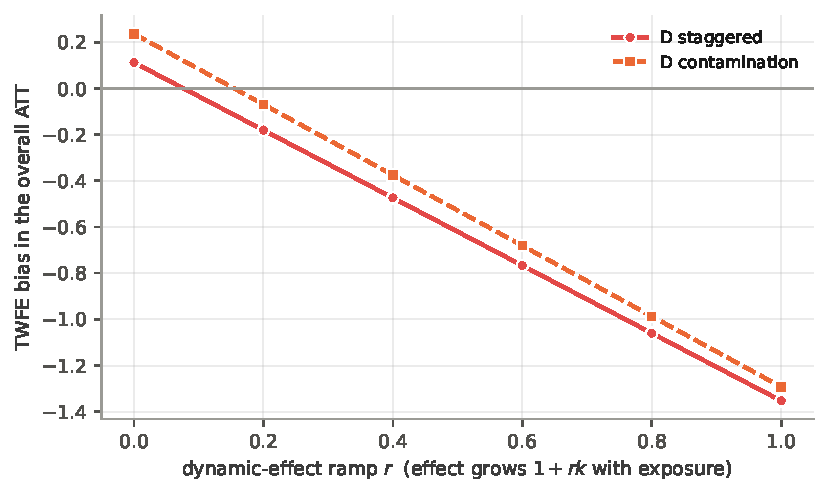
\includegraphics[width=0.92\linewidth]{fig_ramp.pdf}
\caption{Effect paths under the headline staggered and contamination ramps.}
\label{fig:ramp}
\end{figure}

% =============================================================================
\section{Individual CATT-surface results}
% =============================================================================

The paper's distinctive target is an individual heterogeneous effect surface,
not only a scalar ATT. Table~\ref{tab:surface} reports surface RMSE, MAE, MAPE,
and pointwise interval coverage for every available scenario and degree. A
GATT-only estimator is broadcast to treated observations in the relevant cell,
which gives it the natural constant-prediction benchmark.

The surface results show three patterns. First, the plain structured DiD-BCF
surface is substantially better than the broadcast scalar benchmarks in the
canonical designs. Second, grf-DiD is the strongest non-DiD-BCF individual
surface benchmark in most cells. Third, $d=3$ increases the difficulty of the
surface even when scalar bias remains small, because the treatment effect is
now quadratic and non-additive in the effect modifiers. The corrected surface
is generally less efficient than the plain surface because the cell-level
correction is broadcast to individual observations.

\input{tables/tab_surface.tex}

\begin{figure}[htbp]
\centering
\includegraphics[width=0.93\linewidth]{fig_surface.pdf}
\caption{CATT-surface accuracy across the complete available grid.}
\label{fig:surface}
\end{figure}

\begin{figure}[htbp]
\centering
\includegraphics[width=0.93\linewidth]{fig_surface_sweep.pdf}
\caption{CATT-surface accuracy over the available B2 panel-size cells.}
\label{fig:surface-sweep}
\end{figure}

\begin{figure}[htbp]
\centering
\includegraphics[width=0.93\linewidth]{fig_es_methods.pdf}
\caption{Event-study method comparison for the staggered designs.}
\label{fig:es-methods}
\end{figure}

% =============================================================================
\section{Post-correction route audit: structured DiD-BCF and unit random effect}
% =============================================================================

\subsection{What is newly available}

The route file contains the first direct comparison between the two structured
implementations under a common sampling budget. It is a partial B2 ordinary
sweep at $d=1$ with 15 replications per cell. The benchmark rows below use
the current 100-replication benchmark files at $N=200$. These route results
are not substitutes for the complete 100-replication grid, but they answer
the implementation question the full grid cannot answer because it has no
unit-random-intercept output.

\begin{table}[htbp]
\centering
\footnotesize
\caption{Post-correction B2 route comparison at $d=1$, $N=200$.}
\label{tab:route-head}
\begin{tabular}{lllrrrrr}
\toprule
Method & Unit intercept & Summary & $R$ & Bias & RMSE & Cov.95 & Surface RMSE \\
\midrule
DiD-BCF & no & plain & 15 & -0.006 & 0.095 & 1.000 & 0.248 \\
DiD-BCF & no & corrected & 15 & -0.024 & 0.167 & 1.000 & 0.248 \\
DiD-BCF & yes & plain & 15 & -0.009 & 0.091 & 1.000 & 0.241 \\
DiD-BCF & yes & corrected & 15 & -0.031 & 0.159 & 1.000 & 0.241 \\
Callaway--Sant'Anna & n/a & $\gatt(4,4)$ & 100 & -0.031 & 0.221 & 0.980 & 1.069 \\
Gardner & n/a & $\es(0)$ & 100 & -0.047 & 0.179 & 0.980 & 1.072 \\
DoubleML & n/a & $\gatt(4,4)$ & 100 & -0.038 & 0.285 & 0.960 & 1.082 \\
Synthetic DiD & n/a & $\att$ & 100 & -0.023 & 0.169 & 1.000 & 1.062 \\
grf-DiD (Wang) & n/a & $\gatt(4,4)$ & 100 & -0.038 & 0.222 & 0.850 & 0.809 \\
\bottomrule
\end{tabular}
\end{table}

The two route implementations are close in scalar point estimation. The
unit-intercept version has the lower surface RMSE, which is consistent with
the canonical DGP containing a persistent unobserved unit effect. The
benchmark comparison confirms that the surface advantage is not simply a
scalar ATT advantage: the GATT-only competitors are broadcast and the
individual-level grf-DiD benchmark is better than those but remains above the
two DiD-BCF route fits in this small partial run. Coverage is not decisive
because 15 replications make a coverage estimate of 1.000 compatible with a
Monte-Carlo standard error of about $0.055$.

\begin{longtable}{llrrrrr}
\caption{Post-correction B2 route sweep. Entries are bias, RMSE, 95\% coverage,
and CATT-surface RMSE.}\label{tab:route-sweep}\\
\toprule
Unit intercept & Summary & $N$ & Bias & RMSE & Cov.95 & Surface RMSE \\
\midrule
\endfirsthead
\multicolumn{7}{l}{\emph{\footnotesize Table \ref{tab:route-sweep} continued.}}\\
\toprule
Unit intercept & Summary & $N$ & Bias & RMSE & Cov.95 & Surface RMSE \\
\midrule
\endhead
\bottomrule
\endlastfoot
no & plain & 200 & -0.006 & 0.095 & 1.000 & 0.248 \\
no & corrected & 200 & -0.024 & 0.167 & 1.000 & 0.248 \\
yes & plain & 200 & -0.009 & 0.091 & 1.000 & 0.241 \\
yes & corrected & 200 & -0.031 & 0.159 & 1.000 & 0.241 \\
no & plain & 400 & -0.013 & 0.140 & 1.000 & 0.183 \\
no & corrected & 400 & -0.013 & 0.140 & 1.000 & 0.183 \\
yes & plain & 400 & -0.009 & 0.140 & 1.000 & 0.175 \\
yes & corrected & 400 & -0.009 & 0.140 & 1.000 & 0.175 \\
no & plain & 800 & -0.012 & 0.095 & 1.000 & 0.168 \\
no & corrected & 800 & -0.012 & 0.095 & 1.000 & 0.168 \\
yes & plain & 800 & -0.012 & 0.095 & 1.000 & 0.159 \\
yes & corrected & 800 & -0.012 & 0.095 & 1.000 & 0.159 \\
no & plain & 1600 & -0.001 & 0.056 & 1.000 & 0.136 \\
no & corrected & 1600 & -0.001 & 0.056 & 1.000 & 0.136 \\
yes & plain & 1600 & 0.003 & 0.056 & 1.000 & 0.125 \\
yes & corrected & 1600 & 0.003 & 0.056 & 1.000 & 0.125 \\
\end{longtable}
\noindent\emph{Note.} The values at $N=400,800,1600$ are rounded summaries of the
15-replication route output. The corrected and plain point estimates are very
close in this route file; the correction is more visible in posterior spread
than in the displayed point metrics.

\subsection{Interpretation and missing route cells}

The unit-level random intercept is the preferred primary implementation for
the canonical DGP once its full-grid evidence is available, because it targets
the persistent unit-level component directly while preserving the two-way
restriction. The no-unit-intercept structured fit remains necessary as a
sensitivity analysis. The current route file does not support claims about
unit-intercept performance in B1, B2 serial correlation, D staggered adoption,
or $d=2,3$. Those cells must be run before choosing a final primary
specification on the basis of route-specific surface or coverage results.

% =============================================================================
\section{Overall interpretation and remaining work}
% =============================================================================

The complete current structured grid supports four conclusions. First, the
two-way-restricted DiD-BCF point estimates are stable across the canonical B1
and B2 designs, including the transformed nuisance axis and the nonlinear
effect axis. Second, serial correlation at $d=1$ is the setting in which the
posterior correction has the clearest scalar inferential benefit, but that
benefit does not survive the degree axis: at $d=2$ and $d=3$ the corrected
event-study RMSE in the staggered designs exceeds pooled TWFE at every event
time, so the correction cannot currently be recommended outside $d=1$. Third,
the structured
fit handles the cohort-time heterogeneity in the D designs without the pooled
TWFE contamination visible in the Goodman--Bacon decomposition, although the
cell-level table shows that the plain fit pays for this with a concentrated
bias and undercoverage in the late-adopting cohorts that the cell average
hides. Fourth, both DiD-BCF specifications are correctly sized under the sharp
null, the plain fit conservatively so at $0.01$ to $0.05$ and the corrected fit
at $0.03$ to $0.09$, which is within Monte-Carlo error of nominal at 100
replications. On this axis the paper's estimator is better behaved than
grf-DiD, whose null rejection rate reaches $0.25$.

The route audit adds a fifth, narrower conclusion. At $d=1$ in the partial B2
ordinary sweep, the unit random intercept modestly improves the individual
CATT surface and does not materially change scalar bias. This is exactly the
comparison that should guide the next run, but it is not a substitute for
running the unit-intercept route over every B1, B2, and D design and over
$d=1,2,3$.

The next computational block should therefore extend the route file in the
following order. The B1 baseline, strong-confounder, serial-correlation,
selection-on-observables, and null designs should be run first at all three
degrees, because they identify whether the unit effect and correction interact
with the degree axis. Finally, both D designs should be run with the unit
intercept at all three degrees, with scalar GATT, event-study, and individual
surface metrics retained. The sharp-null rejection rate, pointwise CATT
coverage, and surface RMSE should be treated as explicit acceptance criteria,
not as secondary diagnostics.

% =============================================================================
\appendix
\section{Files used and reproducibility}

The DGP and estimator definitions are in
\url{Simulation_Studies_Revision/did_bcf_revision/dgps.py},
\url{Simulation_Studies_Revision/did_bcf_revision/structured.py}, and
\url{didbcf_structured/design.py}. The metric definitions are in
\url{Simulation_Studies_Revision/did_bcf_revision/metrics.py} and the
posterior correction is in
\url{Simulation_Studies_Revision/did_bcf_revision/posterior_correction.py}.

The complete-grid aggregates and generated tables were rebuilt with
\begin{center}
\url{Simulation_Studies_Revision/Results/analysis/aggregate_all.py}\par
\url{Simulation_Studies_Revision/Results/analysis/make_analysis.py}
\end{center}
The generated figures used in this report are
\begin{center}
\url{figures/fig_sweep.pdf}\par
\url{figures/fig_sqrtn.pdf}\par
\url{figures/fig_calibration.pdf}\par
\url{figures/fig_surface.pdf}\par
\url{figures/fig_surface_sweep.pdf}\par
\url{figures/fig_event_study.pdf}\par
\url{figures/fig_ramp.pdf}\par
\url{figures/fig_es_methods.pdf}\par
\url{figures/fig_es_bias.pdf}
\end{center}

The full structured input files are the CSV summaries under \url{DiD_BCF/}.
The B2 ordinary and serial sweeps each contain 100 replications for every
panel size $N\in\{50,100,200,400,800\}$ and degree $d\in\{1,2,3\}$, with both
plain and corrected DiD-BCF summaries. The corresponding DoubleML files were
unpacked from the eight B2 result archives under \url{DoubleML_Colab/} before
the aggregates and tables were rebuilt. The route audit uses only
\url{identification/routes_raw_B2_sweep_lin_1_full.csv}; its 15 replications
per cell are kept separate from the full-grid aggregates. The report should be
recompiled from this directory with two runs of \texttt{pdflatex}.

\end{document}
